\documentclass[portrait,final,a0paper,fontscale=0.277]{baposter}

\usepackage{calc}
\usepackage{graphicx}
\usepackage{amsmath}
\usepackage{amssymb}
\usepackage{relsize}
\usepackage{multirow}
\usepackage{rotating}
\usepackage{bm}
\usepackage{url}
\usepackage{enumitem}


\usepackage{scalefnt}

\usepackage{graphicx}
\usepackage{multicol}

%\usepackage{times}
%\usepackage{helvet}
%\usepackage{bookman}
\usepackage{palatino}

\newcommand{\captionfont}{\footnotesize}

\graphicspath{{images/}{../images/}}
\usetikzlibrary{calc}

\newcommand{\SET}[1]  {\ensuremath{\mathcal{#1}}}
\newcommand{\MAT}[1]  {\ensuremath{\boldsymbol{#1}}}
\newcommand{\VEC}[1]  {\ensuremath{\boldsymbol{#1}}}
\newcommand{\Video}{\SET{V}}
\newcommand{\video}{\VEC{f}}
\newcommand{\track}{x}
\newcommand{\Track}{\SET T}
\newcommand{\LMs}{\SET L}
\newcommand{\lm}{l}
\newcommand{\PosE}{\SET P}
\newcommand{\posE}{\VEC p}
\newcommand{\negE}{\VEC n}
\newcommand{\NegE}{\SET N}
\newcommand{\Occluded}{\SET O}
\newcommand{\occluded}{o}

%%%%%%%%%%%%%%%%%%%%%%%%%%%%%%%%%%%%%%%%%%%%%%%%%%%%%%%%%%%%%%%%%%%%%%%%%%%%%%%%
%%%% Some math symbols used in the text
%%%%%%%%%%%%%%%%%%%%%%%%%%%%%%%%%%%%%%%%%%%%%%%%%%%%%%%%%%%%%%%%%%%%%%%%%%%%%%%%

%%%%%%%%%%%%%%%%%%%%%%%%%%%%%%%%%%%%%%%%%%%%%%%%%%%%%%%%%%%%%%%%%%%%%%%%%%%%%%%%
% Multicol Settings
%%%%%%%%%%%%%%%%%%%%%%%%%%%%%%%%%%%%%%%%%%%%%%%%%%%%%%%%%%%%%%%%%%%%%%%%%%%%%%%%
\setlength{\columnsep}{1.5em}
\setlength{\columnseprule}{0mm}

%%%%%%%%%%%%%%%%%%%%%%%%%%%%%%%%%%%%%%%%%%%%%%%%%%%%%%%%%%%%%%%%%%%%%%%%%%%%%%%%
% Save space in lists. Use this after the opening of the list
%%%%%%%%%%%%%%%%%%%%%%%%%%%%%%%%%%%%%%%%%%%%%%%%%%%%%%%%%%%%%%%%%%%%%%%%%%%%%%%%
\newcommand{\compresslist}{%
\setlength{\itemsep}{1pt}%
\setlength{\parskip}{0pt}%
\setlength{\parsep}{0pt}%
}

%%%%%%%%%%%%%%%%%%%%%%%%%%%%%%%%%%%%%%%%%%%%%%%%%%%%%%%%%%%%%%%%%%%%%%%%%%%%%%
%%% Begin of Document
%%%%%%%%%%%%%%%%%%%%%%%%%%%%%%%%%%%%%%%%%%%%%%%%%%%%%%%%%%%%%%%%%%%%%%%%%%%%%%

\begin{document}

%%%%%%%%%%%%%%%%%%%%%%%%%%%%%%%%%%%%%%%%%%%%%%%%%%%%%%%%%%%%%%%%%%%%%%%%%%%%%%
%%% Here starts the poster
%%%---------------------------------------------------------------------------
%%% Format it to your taste with the options
%%%%%%%%%%%%%%%%%%%%%%%%%%%%%%%%%%%%%%%%%%%%%%%%%%%%%%%%%%%%%%%%%%%%%%%%%%%%%%
% Define some colors

%\definecolor{lightblue}{cmyk}{0.83,0.24,0,0.12}
\definecolor{lightblue}{rgb}{0.145,0.6666,1}

% % Draw a video
% \newlength{\FSZ}
% \newcommand{\drawvideo}[3]{% [0 0.25 0.5 0.75 1 1.25 1.5]
%    \noindent\pgfmathsetlength{\FSZ}{\linewidth/#2}
%    \begin{tikzpicture}[outer sep=0pt,inner sep=0pt,x=\FSZ,y=\FSZ]
%    \draw[color=lightblue!50!black] (0,0) node[outer sep=0pt,inner sep=0pt,text width=\linewidth,minimum height=0] (video) {\noindent#3};
%    \path [fill=lightblue!50!black,line width=0pt] 
%      (video.north west) rectangle ([yshift=\FSZ] video.north east) 
%     \foreach \x in {1,2,...,#2} {
%       {[rounded corners=0.6] ($(video.north west)+(-0.7,0.8)+(\x,0)$) rectangle +(0.4,-0.6)}
%     }
% ;
%    \path [fill=lightblue!50!black,line width=0pt] 
%      ([yshift=-1\FSZ] video.south west) rectangle (video.south east) 
%     \foreach \x in {1,2,...,#2} {
%       {[rounded corners=0.6] ($(video.south west)+(-0.7,-0.2)+(\x,0)$) rectangle +(0.4,-0.6)}
%     }
% ;
%    \foreach \x in {1,...,#1} {
%      \draw[color=lightblue!50!black] ([xshift=\x\linewidth/#1] video.north west) -- ([xshift=\x\linewidth/#1] video.south west);
%    }
%    \foreach \x in {0,#1} {
%      \draw[color=lightblue!50!black] ([xshift=\x\linewidth/#1,yshift=1\FSZ] video.north west) -- ([xshift=\x\linewidth/#1,yshift=-1\FSZ] video.south west);
%    }
%    \end{tikzpicture}
% }

\hyphenation{resolution occlusions}
%%
\begin{poster}%
  % Poster Options
  {
  % Show grid to help with alignment
  grid=false,
  % Column spacing
  colspacing=1em,
  % Color style
  bgColorOne=white,
  bgColorTwo=white,
  borderColor=lightblue,
  headerColorOne=black,
  headerColorTwo=lightblue,
  headerFontColor=white,
  boxColorOne=white,
  boxColorTwo=lightblue,
  % Format of textbox
  textborder=roundedleft,
  % Format of text header
  %eyecatcher=true,
  eyecatcher=true,
  headerborder=closed,
  headerheight=0.1\textheight,
%  textfont=\sc, An example of changing the text font
  headershape=roundedright,
  headershade=shadelr,
  headerfont=\Large\bf\textsc, %Sans Serif
  textfont={\setlength{\parindent}{1.5em}},
  boxshade=plain,
%  background=shade-tb,
  background=plain,
  linewidth=2pt
  }
  % Eye Catcher
  {%
\includegraphics[height=1.0em]{images/CodeCogsEqn.pdf}
  
\includegraphics[height=8.5em]{images/zimt_logo_square_RGB-1024x738.png}
  } 
  % Title
  {\begingroup
    \scalefont{1.0}
      \bf\textsc{Ithaka: a taxonomic classifier \\
      {\vspace{-0.2em} \scalefont{0.7} based on \\} 
      \vspace{0.0em}	
            Bloom filters, and spaced seeds}
   \endgroup
   \vspace{0.06em}}
  % Authors
  {\textsc{Maciej Sykulski, Karel B{\v r}inda, Gregory Kucherov}\\
   {\small macieksk@gmail.com, karel.brinda@univ-mlv.fr, gregory.kucherov@univ-mlv.fr}
   }   
      %\{ Brian.Amberg and Thomas.Vetter \}@unibas.ch}}
  % University logo
  {% The makebox allows the title to flow into the logo, this is a hack because of the L shaped logo.
    
    
\includegraphics[height=8.0em]{images/UPEM_LOGO_SIGNALETIQUE_SMALL.pdf}
  }

%%%%%%%%%%%%%%%%%%%%%%%%%%%%%%%%%%%%%%%%%%%%%%%%%%%%%%%%%%%%%%%%%%%%%%%%%%%%%%
%%% Now define the boxes that make up the poster
%%%---------------------------------------------------------------------------
%%% Each box has a name and can be placed absolutely or relatively.
%%% The only inconvenience is that you can only specify a relative position 
%%% towards an already declared box. So if you have a box attached to the 
%%% bottom, one to the top and a third one which should be in between, you 
%%% have to specify the top and bottom boxes before you specify the middle 
%%% box.
%%%%%%%%%%%%%%%%%%%%%%%%%%%%%%%%%%%%%%%%%%%%%%%%%%%%%%%%%%%%%%%%%%%%%%%%%%%%%%
    %
    % A coloured circle useful as a bullet with an adjustably strong filling
    \newcommand{\colouredcircle}{%
      \tikz{\useasboundingbox (-0.2em,-0.32em) rectangle(0.2em,0.32em); \draw[draw=black,fill=lightblue,line width=0.03em] (0,0) circle(0.18em);}}

      \scalefont{0.9}
%%%%%%%%%%%%%%%%%%%%%%%%%%%%%%%%%%%%%%%%%%%%%%%%%%%%%%%%%%%%%%%%%%%%%%%%%%%%%%
  \headerbox{Metagenomics \& NGS}{name=problem,column=0,row=0}{
%%%%%%%%%%%%%%%%%%%%%%%%%%%%%%%%%%%%%%%%%%%%%%%%%%%%%%%%%%%%%%%%%%%%%%%%%%%%%%

Metagenomics is a powerful approach to study genetic material contained
in environmental samples, which is revolutionized by high-throughput sequencing
technologies. Taxonomic classification of metagenomics data sets is a common step in analysis, a step for which computational cost becomes prohibitive with the growth of metagenomic datasets.

Approaches using sequence alignment algorithms, often based on the Burrows-Wheeler transform, such as Kaiju\cite{kaiju}, Centrifuge\cite{centrifuge}, compete successfully with k-mer based alignment-free comparison methods such as Kraken\cite{kraken}, Clark\cite{clark}. Improvements to k-mer based approaches include: extending contiguous k-mers with spaced seeds \cite{sseed}\cite{clark}, using Bloom filters as an underlying data structure for storing k-mers.\cite{trie}

%     {\bf Metagenomics} is a powerful approach to study genetic
% content of environmental samples, which has been strongly promoted
% by NGS technologies.
% %
% 
% For large-scale metagenomic projects
% %, alignment-based approaches appear unfeasible, and 
% alignment-free methods are used.
% %aligning multimillion read sets against thousands
% %of genomes remains computationally difficult even with optimized
% %tools. 
% %
% To cope with massive data,
% %involved in modern metagenomic projects, 
% recent tools 
% %(Ames et al., 2013; Wood and
% %Salzberg, 2014) 
% (LMAT \cite{lmat}, Kraken \cite{kraken})
% rely on the analysis of {\bf k-mers} (words of fixed size)
% shared between the
% {\bf read} to be classified, and {\bf reference genomes}.

   \vspace{0.3em}
 }



%%%%%%%%%%%%%%%%%%%%%%%%%%%%%%%%%%%%%%%%%%%%%%%%%%%%%%%%%%%%%%%%%%%%%%%%%%%%%%
  \headerbox{References}{name=references,column=0,above=bottom}{
%%%%%%%%%%%%%%%%%%%%%%%%%%%%%%%%%%%%%%%%%%%%%%%%%%%%%%%%%%%%%%%%%%%%%%%%%%%%%%
    \smaller
    \bibliographystyle{ieee}
    \renewcommand{\section}[2]{\vskip 0.05em}
      \begin{thebibliography}{1}\itemsep=-0.01em
      \setlength{\baselineskip}{0.4em}
%       \bibitem{noe:coverage}
%          L.~No{\'e}, D.~E.~K.~Martin.
%          \newblock {A} coverage criterion for spaced seeds and its
%         applications to support vector machine string kernels and k-mer
%       distances. 
%       \newblock In Journal of Computational Biology 21, 2014.
%       %      
\bibitem{kaiju} %[1]
Menzel,~P, Ng~Kim~Lee, Krogh~A
\newblock Fast and sensitive taxonomic classification for metagenomics with Kaiju.
\newblock Nat Commun 7, Nature Publishing Group, apr 2016, 
      
\bibitem{centrifuge} Kim~D, Song~L, Breitwieser~F~P, Salzberg~S %[2]
\newblock Centrifuge: rapid and sensitive classification of metagenomic sequences
\newblock Genome 1.2: 2.

\bibitem{kraken} %[3]
      Wood,~D.~E. and Salzberg,~S.~L.
      \newblock Kraken: ultrafast metagenomic sequence classification using exact alignments. 
      \newblock In Genome Biol., 15(3), R46. (2014)

\bibitem{clark} Ounit~R, Lonardi~S, %[4,6]
\newblock Higher classification sensitivity of short metagenomic reads with CLARK-S
\newblock bioRxiv 053462; doi: http://dx.doi.org/10.1101/053462

\bibitem{sseed} B{\v r}inda,~K,Sykulski~M, Kucherov~G.  %[5]
\newblock Spaced seeds improve k-mer-based metagenomic classification.
\newblock Bioinformatics 31.22 (2015): 3584-3592.

\bibitem{trie} Holley~G, Wittler~R, Stoye~J.  %[7]
\newblock Bloom Filter Trie: an alignment-free and reference-free data structure for pan-genome storage. 
\newblock Algorithms for Molecular Biology. 2016;11: 3.      
            
      \end{thebibliography}
 
 \vspace{-1.5em}
 
 \hspace{-2.0em}
  \begin{minipage}{\textwidth}
  \begin{minipage}{0.80\linewidth}
  %  \indent{}
  %The source code \\ and the manual \\ are available at   
   {\smaller 
  \url{https://github.com/gregorykucherov/ithaka}\\
  \url{http://seed-kraken.readthedocs.org} 
  %\url{http://arxiv.org/abs/1502.06256}
   }
  \end{minipage}\hfill%
  \begin{minipage}{0.20\linewidth}
  %\hfill
\includegraphics[width=\linewidth]{images/qr-seed-kraken-rea-crop.pdf}
  \hfill
\includegraphics[width=\linewidth]{images/qrcode-ithaka.png}
  \end{minipage}
  \end{minipage}
   \vspace{0.3em}
  }



%%%%%%%%%%%%%%%%%%%%%%%%%%%%%%%%%%%%%%%%%%%%%%%%%%%%%%%%%%%%%%%%%%%%%%%%%%%%%%
  \headerbox{Spaced Seeds}{name=method,column=0,below=problem}{
%%%%%%%%%%%%%%%%%%%%%%%%%%%%%%%%%%%%%%%%%%%%%%%%%%%%%%%%%%%%%%%%%%%%%%%%%%%%%%

  A {\bf spaced seed} is a pattern over alphabet 
  $A=\{\textbf{\#}, \textbf{--}\}$, where\\
  $\#$ matching position,\, $-$ don't care position.
\vspace{-0.5em}  
  \noindent{\begin{center}
	    
\includegraphics[height=2.5em]{images/CodeCogsEqn.pdf}
	    %{images/seed_expl-crop.pdf}
	    \end{center}}
\vspace{-0.8em}
% A seed acts as a mask for comparing short oligonucleotides.
% The number of $\textbf{\#}$'s in a seed, called {\em weight},
% defines the number k of matching nucleotides. 
% In the above example k = 4, seed span = 6,
% and the matching (spaced) k-mer is ${\bf ACTC}$ signifying a {\bf hit}.

Previously, we demonstrated that spaced seeds allow for a better
   classification of NGS reads coming from a genome $G$ between two
  other genomes $G_1$ and $G_2$ of the same genus.\cite{sseed}
\\  
 {\bf Coverage} is a number of aligned pairs covered 
 by $\textbf{\#}$ from a spaced seed matches while sliding over an alignment 
 (=4 above). 
 \\
{\bf Coverage pattern} is the pattern of matches (hits) of a seed over an alignment.
\\
{\bf The NP-HARD PROBLEM:}  Assume a read $f$ comes from genome $g$.
For a given seed, computing $e_{f,g}$ -- a minimal number of errors(mutations) in fragment $f$, given the {\em coverage pattern} of the read $f$ with hits to $g$ is NP-hard. In other words, answering what is the minimal number of errors in a fragment $f$ which guarantees a certain coverage pattern (eg. found by Ithaka query) turns out to be an instance of 0-1 integer programming (an NP-complete problem). We programmed our solution using {\em coin-Cbc} integer programming library. In practice, it works fast on reads with high coverage, and slows down significantly on reads with low coverage (then heuristic is preferred).
   \vspace{0.3em}
  }

% 
% %%%%%%%%%%%%%%%%%%%%%%%%%%%%%%%%%%%%%%%%%%%%%%%%%%%%%%%%%%%%%%%%%%%%%%%%%%%%%%
%   \headerbox{Contributions}{name=contribution,column=0,below=method, above=references}{
% %%%%%%%%%%%%%%%%%%%%%%%%%%%%%%%%%%%%%%%%%%%%%%%%%%%%%%%%%%%%%%%%%%%%%%%%%%%%%%
% %\begin{itemize}
% $\bullet$\,We showed that spaced seeds can improve success
%   rate of binary classification of alignments into two categories, each
%   defined by a specific mismatch rate.
%   %Here the classification is done
%   %through ``querying'' an alignment using a seed as a mask and
%   %reporting whether the seed applies at a given position. 
%   For example,
%   in discriminating between alignments of length 100 with mismatch
%   rate $0.2$ and $0.3$, a spaced seed of weight 16 achieves 63\% of
%   success while a contiguous seed of the same weight achieves only
%   40\%. 
% 
% $\bullet$\,We demonstrated that spaced seeds allow for a better
%   classification of NGS reads coming from a genome $G$ between two
%   other genomes $G_1$ and $G_2$ of the same genus. 
%   %Here reads are
%   %classified according to the phylogenetic distance
%   %between $G$ and $G_1$ and $G$ and $G_2$ respectively. We established that correct classification is obtained
%   %with seeds of weight 16 and more, while seeds of weight 14 are
%   %insufficient. 
% 
% $\bullet$\,We analyzed how well different estimators (coverage/hit-number
%   combined with spaced/contiguous seed) correlate with the alignment
%   quality, also on real genomes. %(center panel).
%   %, by measuring Spearman's rank correlation
%   %coefficient and mutual information coefficient.
%     
% %$\bullet$\,We compare spaced and contiguous seeds through
% % large-scale metagenomics experiments (right panel).
% $\bullet$\,We demonstrated that spaced seeds can improve the sensitivity-selectivity trade-off in large-scale metagenomics experiments ({\sc seed-Kraken} panel).
% %
% %\noindent{\bf Results:}
% %     Within this general framework, we show that spaced
% % seeds provide a significant improvement of classification capacity as
% % opposed to traditional contiguous k-mers. We support this thesis
% % through a series a different computational experiments, including
% % simulations of large-scale metagenomic projects.
%    
% % %To study this, we implemented the
% % %following experimental setup. 
% % %
% % Using {\sc dwgsim} read simulator
% % %(\url{http://github.com/nh13/DWGSIM}), 
% % we generate single-end
% % {\sc Illumina}-like reads from genome $G$. 
% % %In all experiments, 
% % We assumed
% % 1\% of base mutations (substitutions only), and 2\% of sequencing
% % errors. 
% % %({\sc dwgsim} options \texttt{-e 0.02 -r 0.01 -R 0}). 
% % Given a seed  $k$-mers of $G_1$ and $G_2$ are indexed.
% % %to support existence queries only. 
% % For each read, all $k$-mers are
% % queried against $G_1$ and $G_2$ and corresponding counts $C_1$ and
% % $C_2$ are computed. If $C_1>C_2$ (resp. $C_1<C_2$), the read is classified to be closer
% % to $G_1$ (resp. $G_2$), otherwise a tie is reported. 
% % 
% % {\noindent
% % \scriptsize 
% % % \begin{table}
% \caption{\small Classification of {\em Bacillus thuringiensis} reads
%   against {\em Bacillus anthracis} and {\em Bacillus cereus} genomes. Each entry contains a pair ``Fraction (in \%) of reads
%   classified closer to {\em B.anthracis}\, /\,Fraction of reads
%   classified closer to {\em B.cereus} ''. Spaced seeds used are
%   shown in Table~\ref{smeg_gil_van}.\label{thur_anth_cer}}
% \centering
\begin{tabular}{|r|c|c|c|c|}%c|}
\hline
& \multicolumn{4}{c|}{weight}\\
\cline{2-5}
                        & 14            & 16         & 18        & 20       
                        \\%& 22\\
                        
\hline
  contig hit nb    & 83 / 14 & 81 / 11 & 79 / 09 & 77 / 08 \\%& 76 / 08\\
  contig cover     & 78 / 17 & 80 / 12 & 79 / 09 & 77 / 08 \\%& 76 / 08\\
\hline
  spaced hit nb    & 83 / 13 & 82 / 11 & 80 / 09 & 79 / 09 \\%& 79 / 08\\
  spaced cover    & 80 / 15 & 81 / 11 & 80 / 09 & 79 / 09 \\%& 79 / 08\\
\hline
\end{tabular}
% \end{table}


% % }  
% % \vspace{0.3em}
% % % \caption{\small 
% % Classification of {\em Bacillus thuringiensis} reads
% %   against {\em Bacillus anthracis} and {\em Bacillus cereus} genomes. Each entry contains a pair ``Fraction (in \%) of reads
% %   classified closer to {\em B.anthracis}\, /\,Fraction of reads
% %   classified closer to {\em B.cereus} ''.
% % %
% \vspace{0.3em}
%   }



%%%%%%%%%%%%%%%%%%%%%%%%%%%%%%%%%%%%%%%%%%%%%%%%%%%%%%%%%%%%%%%%%%%%%%%%%%%%%%
\headerbox{2outof3 Index}{name=results,column=1,span=1,row=0}{
  %%%%%%%%%%%%%%%%%%%%%%%%%%%%%%%%%%%%%%%%%%%%%%%%%%%%%%%%%%%%%%%%%%%%%%%%%%%%%%
Consider a binary tree with a 
  
  
{\bf Ithaka 2outof3 index} is comparable in size to Krakens: 67GB for bacterial and archaeal, but
\vspace{-0.7em}
\begin{itemize}[leftmargin=*]
\setlength\itemsep{-0.2em}
\item it requires 24 GB to be build (although it builds much faster when more is available) (Kraken requires 120GB to build the db)
\item it requires <24 GB to run
\item it contains complete taxonomic information about k-mers, not only LCAs  
\end{itemize}
% We generated a set of {\sc Illumina}-like single-end reads:
% we've selected random substrings of 
% {\em M.tuberculosis} genome
% %$G$
% of length $L=100$ and
% introduced $k$ mismatch errors, with $k$ random between $1$ and $20$.
% For each read, we computed: {\bf number of hits} and {\bf coverage}
% to the genome under a given seed.
% %This experiment has been applied to {\em M. tuberculosis} genome, 
% A typical plot error vs score (seed weight 20).
% \noindent\begin{tabular}{@{\hspace{0.0em}}c@{\hspace{0.0em}}c@{\hspace{0.0em}}}
% Hits & Coverage\\
% 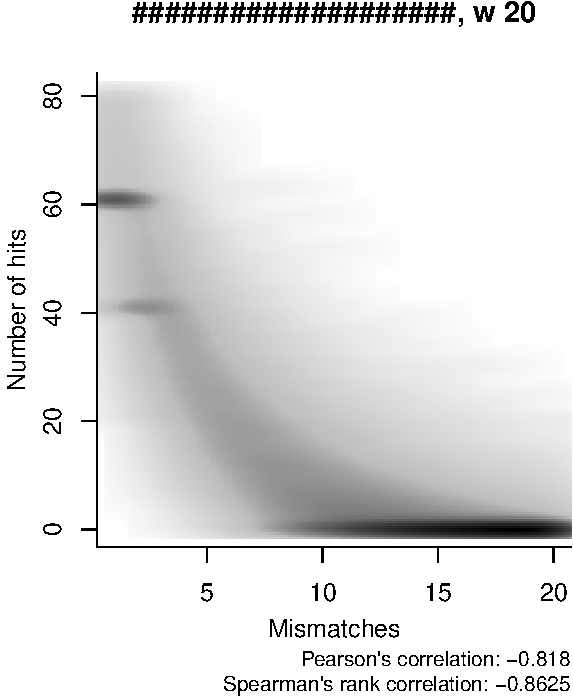
\includegraphics[width=0.49\linewidth]{images/3.3/Myco-w20-cont-hit-scatter-crop.pdf} &
% 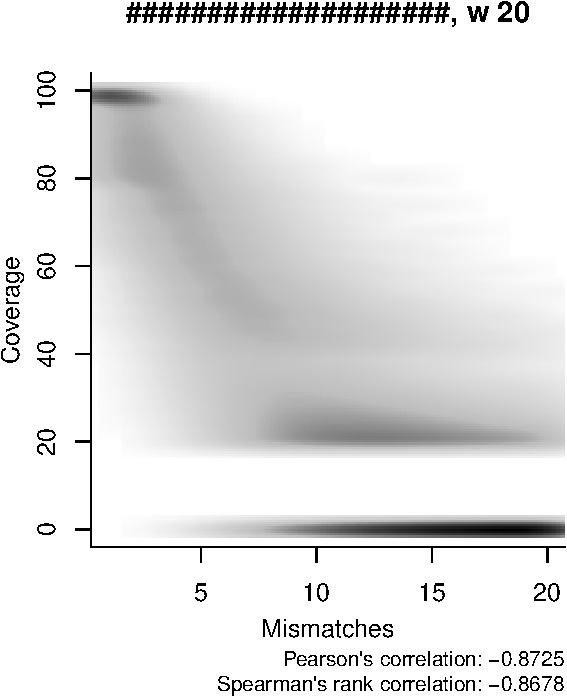
\includegraphics[width=0.49\linewidth]{images/3.3/Myco-w20-cont-cover-scatter-crop.pdf} \\%[2em]
% 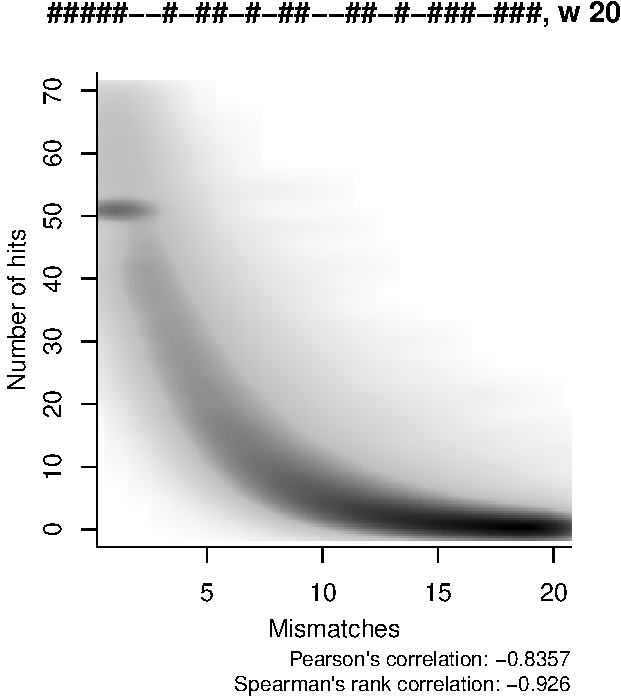
\includegraphics[width=0.49\linewidth]{images/3.3/Myco-w20-spaced-hit-scatter-crop.pdf} &
% 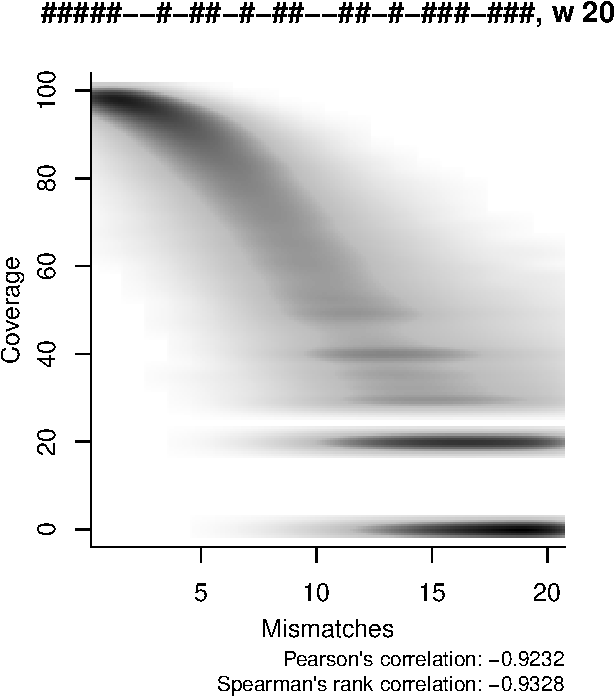
\includegraphics[width=0.49\linewidth]{images/3.3/Myco-w20-spaced-cover-scatter-crop.pdf} \\%[2em]
% %\begin{sideways}{\makebox[0.32\linewidth][c]{Flank of a giraffe}}\end{sideways} & 
% %\includegraphics[width=0.40\linewidth]{candidates_giraffes_flank_bg}&
% %\includegraphics[width=0.40\linewidth]{candidates_giraffes_flank_no_bg}\\
% \end{tabular}
% {\bf Spaced seeds}
% exhibit a better correlation between errors and score, while
% {\em contiguous seeds} plots are more blurred.
% \vspace{-1.0em}
%      \begin{multicols}{1}
%      Hit number (left plots) and coverage (right plots) depending
% 	on the number of mismatches in randomly generated reads. Seed is
% 	shown above the plot, and Spearman's and Pearson's correlations are
% 	shown below. Grayscale shows the density of
% 	reads. Experiments made on {\em M.tuberculosis} 
% 	genome.
% %     Between one and three user clicks were needed to achieve accurate tracking for
% %       the head sequence. Note the correct handling of the occluded ear, which
% %       required only a single click. 
% % 
% %       The eye of the running giraffe required eight user interactions, of which three
% %       marked occlusions. 
%        \end{multicols}
\vspace{0.3em}
}


%%%%%%%%%%%%%%%%%%%%%%%%%%%%%%%%%%%%%%%%%%%%%%%%%%%%%%%%%%%%%%%%%%%%%%%%%%%%%%
\headerbox{Ithaka Toolchain and Performance}{name=speed,column=1,span=2,below=results,above=bottom}{ %,bottomaligned=background model}{
  %%%%%%%%%%%%%%%%%%%%%%%%%%%%%%%%%%%%%%%%%%%%%%%%%%%%%%%%%%%%%%%%%%%%%%%%%%%%%%

% We modified  {\sc
%     Kraken} software \cite{kraken} to make it work with
%   spaced seeds rather than with contiguous seeds only.
%Our implementation allows the user to specify a spaced seed as a parameter. 
% For a set of genomes, a database of spaced $k$-mers matching a user-selected seed is constructed. 
%
\hspace{-1em}
\begin{minipage}{0.46\textwidth}
{\bf Ithaka tool chain:}
\vspace{-0.7em}
\begin{itemize}[leftmargin=*]
\setlength\itemsep{-0.2em}
\item ithaka-build.py -- indexing fasta files, taxonomic tree binarization, creating of {\bf 2outof3 index}.
% I think most things are done there, and the process cannot be easily improved, and since this is a rare operation, there is no urgent need to. Building full Bacteria index + HMP database (90GB result, 20GB largest BF) takes approximately 36 hours on 24 cores. One problem here is that during indexing, sequences with gi numbers which do not map to taxonomic id's are simply omitted, and this happens hundreds of times or Bacteria db.
\item ithaka-query.py -- querying the index with a set of reads. 
%To be competitive still needs improvements described below, it's slow.
\item ithaka-assigment.py -- 2 steps:
\vspace{-1em}
\begin{itemize}[leftmargin=0.5em]
\setlength\itemsep{-0.2em}
\item samtoerr -- computing error counts from coverage (NP-hard), 
% and this is now slow for reads with low coverage (40min for >2mln alignments from 50K reads sample) This needs either rewriting to some greedy heuristic, some prefiltering, or both.
\item Expectation Maximization(EM) -- taxonomic abundance estimation, and read assignment (blazing fast: 1000 iterations of 50K reads (>2 million alignments) in <10 seconds)
\end{itemize}
\end{itemize}
\vspace{-0.7em}
%
% This is mostly done, it's blazing fast  Here possible improvements are: heuristic computation of P(f|g) which takes hitcounts into account (first draft done), heuristic prior to \alpha_g which reduces assignments to genomes with very low representation (I experimented with this), better setup of parameters like seq_error_prob, earth_kmer_abundance. However, I have a following observations:
% -- whether error_probability coefficient is 0.01 or 0.001  doesn't seem to change the results much, if the earth_kmer_abundance coefficient is large enough.
% -- lowering the earth_kmer_abundance coefficient (i.e. increasing the probability of assigning a read as unknown) can increase precision, at the cost of sensitivity. (at the family level Ithaka reaches 0.994 precision with 0.78 sensitivity)
%
{\bf Possible improvements to ithaka-query.py}:
In development implementation (partially in C++) is still slow: ~700 reads (of 220-250len) per second. This can be easily sped up 4x by moving totaly to C++.
% which recomputes hashes from reads for every Bloom filter tested. According to below gprof-iler output, this could be relatively easily sped up by a factor of ~4x.
%   %   cumulative   self              self     total           
%  time   seconds   seconds    calls  us/call  us/call  name    
%  47.37      0.27     0.27  1246416     0.22     0.22  compress_kmer
%  24.56      0.41     0.14  1246416     0.11     0.43  Bloom::query
%  19.30      0.52     0.11  9970024     0.01     0.01  MurmurHash3_x64_128
%   3.51      0.54     0.02  1246253     0.02     0.10  compute_hashes
Further speed up is not possible without cache optimization because 25\% of time is spend on querying Bloom filter bitmap: it's the time to access memory with cache misses, the access is random. Effective implementation using {\em "cache blocking"} is possible (10x, total 40x speedup).
% 
% This could be sped up by sorting the all the queried bits numbers, and querying them in order. The trade off would be the sorting time (but this could be done once at the beginning for all reads), and then assembling the responses back into kmer queries, which would again meet with the problem of cache misses (if there are many reads/kmers). This could be mitigated using "cache blocking".
% 
% The competition operates at the speeds of 20x to 80x faster than current Ithaka's 700rps. (see chart below from Kajiu paper) I suspect that cache optimization can give a speed up of a factor ~10x or more. The total speed up can be >40x, but it requires some serious programming work.


{\bf Performances} of classification of {\sc seed-Kraken}\cite{sseed} and {\sc Ithaka} (with spaced seeds), and original {\sc Kraken}, 
were computed on simulated metagenomes (primarily used in \cite{kraken}):    
    MiSeq (10 bacterial genomes, average error rate), 
    Charted are genus precision (positive predictive value) against genus sensitivity (rate of correct assignments). Varying are {\em k-mer length}, and its spaced seed equivalent {\em seed weight}, while the {\em seed span} (not indicated) varies from 31 to 40.
Ithaka marks {\em black}: only leaves(genomes) fed to EM; {\em blue}: also inner nodes fed to EM (precision at cost of sensitivity).
    
%\ \\
%\vspace{0.3em}
%
% {\sc seed-Kraken} outperforms original {\sc Kraken} in sensitivity/precision trade-off (ROC curve characteristics) at the classification levels of genus, and family.
%
%
\end{minipage} 
\hspace{-3em}
\begin{minipage}{0.65\textwidth}
\centerline{
\noindent\begin{tabular}{@{\hspace{0.0em}}c@{\hspace{0.0em}}}
%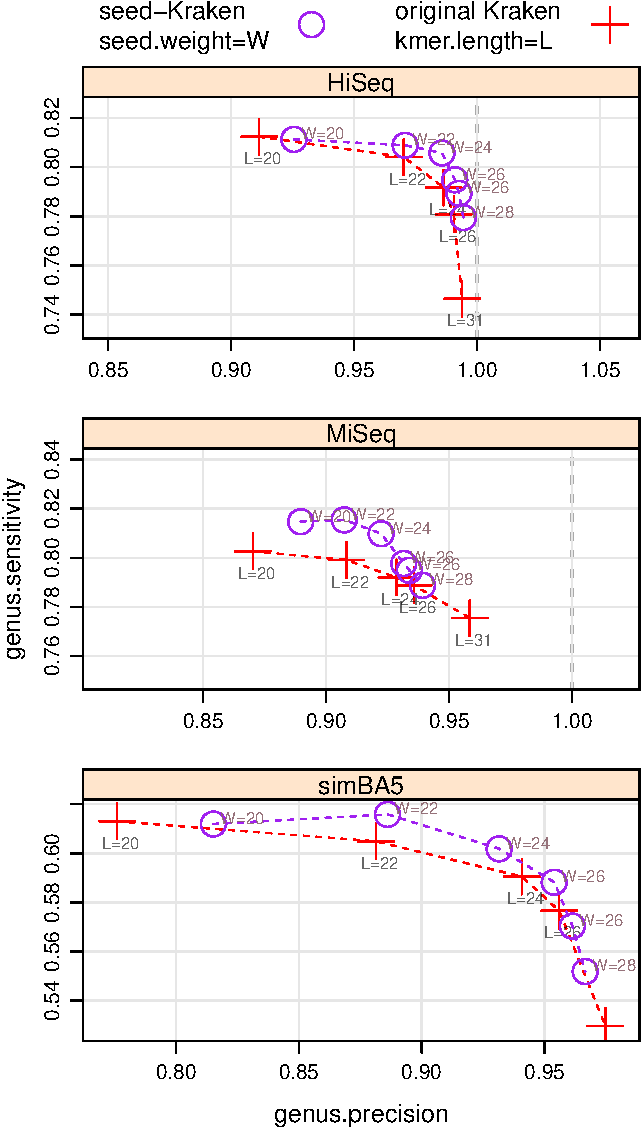
\includegraphics[width=\linewidth,keepaspectratio]{images/seed-kraken_plt1_bioinfo-crop.pdf}\\
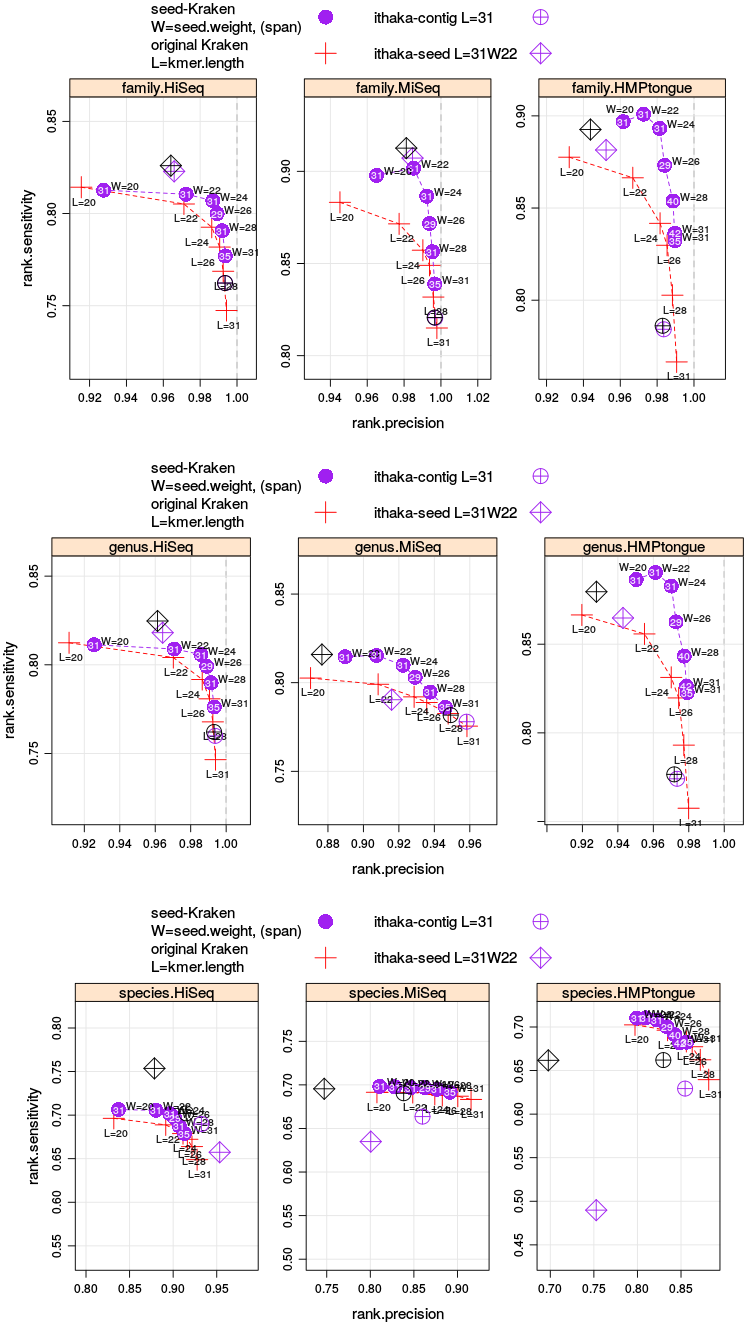
\includegraphics[height=0.41\textheight,keepaspectratio]{images/ithaka_first_results_miseq_fixed.png}\\
\end{tabular}
}
\end{minipage}

  \vspace{0.3em}
 }



%%%%%%%%%%%%%%%%%%%%%%%%%%%%%%%%%%%%%%%%%%%%%%%%%%%%%%%%%%%%%%%%%%%%%%%%%%%%%%
  \headerbox{EM abundance estimation and assignment}{name=background_model,column=2,row=0,span=1,above=speed}{%{name=background model,column=1,below=results,above=bottom}{
%%%%%%%%%%%%%%%%%%%%%%%%%%%%%%%%%%%%%%%%%%%%%%%%%%%%%%%%%%%%%%%%%%%%%%%%%%%%%%
EM solves two problems at once: abundance estimation, and assignment.
EM maximizes likelihood as a function of two types of variables:
\vspace{-1em}
\begin{enumerate}[leftmargin=*]
\setlength\itemsep{-0.2em}
\item abundances  $\alpha_g$  such that  $\sum_{g\in G} \alpha_g =1$  correspond to proportion of reads from the whole sample which belong to genome $g$. Here $G$ is the set of all genomes plus $U$ category of unknown/unclassified reads.
\item categorical assignment indicator 0-1 variables $y_{f,g}$​ which if equal to 1 mean that read $f$ comes from a genome(or category) $g$. Matrix of these variables is sparse – most of them are 0 – since we only consider  $y_{f,g}$ non zero if there are some hits from genome $g$ in fragment $f$.  
$\sum_{g \in G} y_{f,g} = 1$
\end{enumerate}
\vspace{-0.5em}
The {\bf total likelihood} is proportional to
\vspace{-0.5em}
%\begin{align}
$$\left(\prod_{f \in F} \prod_{g \in G} P(f\|g)^{y_{f,g}} \alpha_{g}^{y_{f,g}} \right) \times P_{prior}(\alpha)$$
%\end{align}
%\vspace{-0.5em}
$P_{prior}(\alpha)$ is the conjugate prior distribution to categorical distribution, which is Dirichlet distribution.\\
{\bf Expectation step} goes over $y_{f,g}$​ variables (with $\alpha_g$ set)\\
{\bf Maximization step} goes over  $\alpha_g$  variables (with $y_{f,g}$​ set).

$P(f\|g)$ is given, it's probability of obtaining fragment $f$ assuming it comes from genome $g$, it depends on 
$\frac{1}{\text{kmer\_richness\_of\_g}}$.
One proposal for it depends also on $e_{f,g}$ -- a minimal number of errors/mutations in fragment $f$, given the coverage pattern (see NP-HARD, left panel).

% An accurate mapping of a read to a corresponding clade
% requires estimating its distances to each of the genomes.
% 
% % With this motivation, we studied how
% % well the measured counts correlate with the alignment score. 
% 
% For a fixed minimal identity rate $p_{id}$, 
% we randomly sampled gapless alignments of length
% $100$ with identity rate from interval $[p_{id}..1]$, and
% collected pairs (number of mismatches, score), 
% where 'score' stands for either {\bf number of hits}, or {\bf coverage} of a given seed. For these data, we plot Spearman's rank correlation.
% \vspace{0.5em}
% 
% \noindent\begin{tabular}{@{\hspace{0.0em}}c@{\hspace{0.0em}}}
% 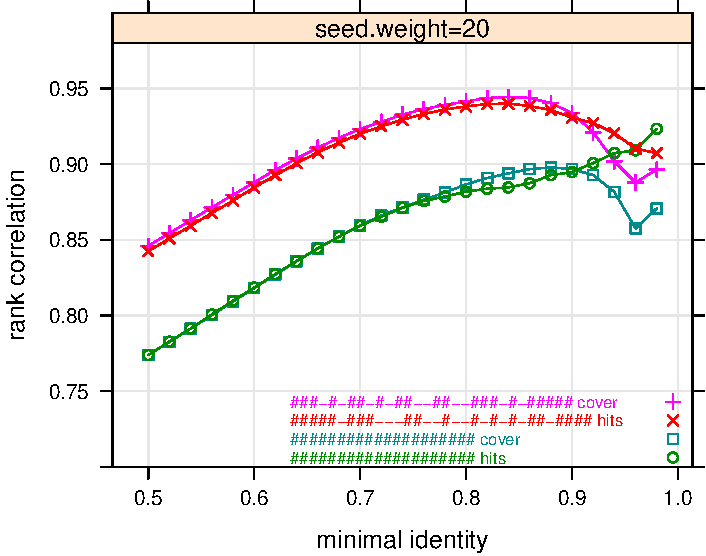
\includegraphics[width=\columnwidth]{images/3.2/rank-cor-seed-weight-20-crop.pdf} \\
% \end{tabular}
% 
% 
% A typical result, corresponding to seed weight 22, is shown in Figure~\ref{spearman}. 
% It implies that when the identity rate of alignments takes a large
% range of values (minimal id rate smaller than $\approx 0.9$), 
% spaced seeds yield a significantly higher correlation than
% contiguous seeds, for both hit-number and coverage
% counts. Furthermore, the coverage count slightly outperforms the
% hit-number count, especially for spaced seeds and larger weights. 
% 
% For high-similarity alignments, however, the picture changes: the coverage
% count loses its performance, with its correlation value sharply
% decreasing. Furthermore, the
% correlation of hit-number goes down for spaced seeds as well, while
% it continues to grow for contiguous seeds ending up by reaching and
% even slightly outperforming the one for spaced seed. 
% % These phenomena are due to combinatorial reasons: when the number of
% % mismatches is small, the number of hits of a contiguous seed
% % correlates very well with the number of mismatches, compared to a
% % spaced seed. 
% This is due to a larger span of spaced seeds and to their 
% combinatorial properties that cause the hit number values to be less
% sharply concentrated at certain values, and therefore to be less well
% correlated with the number of mismatches. 
% 
%  In conclusion, spaced seeds provide a much better
%  distance estimator for alignments whose score ranges over a large interval. For
%  very high-scoring alignments (${>95\%}$ of identity), the hit number of
%  contiguous seed becomes a better estimator. 
%The superiority of
%hit-number over coverage for high-scoring alignments has also
% been reported in \citep{pmid25393923}. Along with Spearman's
% correlation, we also made an analysis of mutual information computed
% on the same data (data not shown) that confirmed the above conclusions.  
 \vspace{0.3em}
  }

% %%%%%%%%%%%%%%%%%%%%%%%%%%%%%%%%%%%%%%%%%%%%%%%%%%%%%%%%%%%%%%%%%%%%%%%%%%%%%%
%   \headerbox{Source on Github, Links}{name=source,column=2,below=background_model}{
% %%%%%%%%%%%%%%%%%%%%%%%%%%%%%%%%%%%%%%%%%%%%%%%%%%%%%%%%%%%%%%%%%%%%%%%%%%%%%%
%   \noindent
%   \begin{minipage}{\linewidth}
%   \begin{minipage}{0.65\linewidth}
%     \indent{}
%   The source code \\ and the manual \\ are available at 
%   \end{minipage}\hfill%
%   \begin{minipage}{0.35\linewidth}
%   %\hfill
\includegraphics[width=\linewidth]{images/qr-seed-kraken-rea-crop.pdf}
%   \hfill
\includegraphics[width=\linewidth]{images/qr-github-com-crop.pdf}
%   \end{minipage}
%   \end{minipage}
%   {\small \\ \ \\
%   \url{http://seed-kraken.readthedocs.org} \\
%   \url{http://github.com/gregorykucherov/spaced-seeds-for-metagenomics}\\
%   \url{http://arxiv.org/abs/1502.06256}
%   }
%   %\\ \hfill
\includegraphics[height=0.5\linewidth]{images/qr-seed-kraken-rea.pdf}
%   }

% %%%%%%%%%%%%%%%%%%%%%%%%%%%%%%%%%%%%%%%%%%%%%%%%%%%%%%%%%%%%%%%%%%%%%%%%%%%%%%
%   \headerbox{A Future Direction}{name=questions,column=1,span=1,below=background model,above=bottom}{
% %%%%%%%%%%%%%%%%%%%%%%%%%%%%%%%%%%%%%%%%%%%%%%%%%%%%%%%%%%%%%%%%%%%%%%%%%%%%%%
%     We incorporated a background model, where a click informs us not only that `this is how the
%     patch looks like', but also for the rest of the frame, `this is how the patch
%     does not look like'. 
%     
%     Can we also \emph{efficiently} use a background tracks model, allowing us
%     to reason, `this would be a good track, but part of it can be better
%     explained by tracking another point'.
%    \vspace{0.3em}
%   }


\end{poster}

\end{document}








Ithaka tool chain

Generally the Ithaka tool chain is:
* ithaka-build.py - indexing fasta files, binarization, and creating 2outof3 index.
I think most things are done there, and the process cannot be easily improved, and since this is a rare operation, there is no urgent need to. Building full Bacteria index + HMP database (90GB result, 20GB largest BF) takes approximately 36 hours on 24 cores. One problem here is that during indexing, sequences with gi numbers which do not map to taxonomic id's are simply omitted, and this happens hundreds of times or Bacteria db.

* ithaka-query.py - querying the index. To be competitive still needs improvements described below, it's slow.

* ithaka-assigment.py - these are 2 steps: first is 
** samtoerr - computing error counts from coverage (NP-hard), and this is now slow for reads with low coverage (40min for >2mln alignments from 50K reads sample) This needs either rewriting to some greedy heuristic, some prefiltering, or both.
** EM - expectation maximization. This is mostly done, it's blazing fast (1000 iterations of 50K reads (>2 million alignments) in <10 seconds). Here possible improvements are: heuristic computation of P(f|g) which takes hitcounts into account (first draft done), heuristic prior to \alpha_g which reduces assignments to genomes with very low representation (I experimented with this), better setup of parameters like seq_error_prob, earth_kmer_abundance. However, I have a following observations:
-- whether error_probability coefficient is 0.01 or 0.001  doesn't seem to change the results much, if the earth_kmer_abundance coefficient is large enough.
-- lowering the earth_kmer_abundance coefficient (i.e. increasing the probability of assigning a read as unknown) can increase precision, at the cost of sensitivity. (at the family level Ithaka reaches 0.994 precision with 0.78 sensitivity)

-- Improvements to ithaka-query.py
Currently it processes ~700 reads (of 220-250len) per second.
This is slow, partially due to inefficient implementation which recomputes hashes from reads for every Bloom filter tested. According to below gprof-iler output, this could be relatively easily sped up by a factor of ~4x.
  %   cumulative   self              self     total           
 time   seconds   seconds    calls  us/call  us/call  name    
 47.37      0.27     0.27  1246416     0.22     0.22  compress_kmer
 24.56      0.41     0.14  1246416     0.11     0.43  Bloom::query
 19.30      0.52     0.11  9970024     0.01     0.01  MurmurHash3_x64_128
  3.51      0.54     0.02  1246253     0.02     0.10  compute_hashes
Further speed up is not possible without cache optimization because 25% of time is spend on querying Bloom filter bitmap, and this is simply the time to access memory (with cache misses, since the access is completely random).
This could be sped up by sorting the all the queried bits numbers, and querying them in order. The trade off would be the sorting time (but this could be done once at the beginning for all reads), and then assembling the responses back into kmer queries, which would again meet with the problem of cache misses (if there are many reads/kmers). This could be mitigated using "cache blocking".

The competition operates at the speeds of 20x to 80x faster than current Ithaka's 700rps. (see chart below from Kajiu paper) I suspect that cache optimization can give a speed up of a factor ~10x or more. The total speed up can be >40x, but it requires some serious programming work.

​

Ithaka experiment results​

This is a bit quagmire. One reason is that gi number to taxonomic id mapping is changing (ftp://ftp.ncbi.nih.gov/pub/taxonomy/). It did change since May, or January. I spotted that one of the 10 MiSeq dataset bacterias: Enterobacter_cloacae_NCTC_9394_uid197202 was dropped in preprocessing because it's gi number was no longer in the database. 
>gi|479270911|ref|NC_021046.1| Enterobacter cloacae subsp. cloacae NCTC 9394 draft genome
The above gi|479270911 is no longer in database, and NCBI page reports different taxid: 295095013 .
Missing bacteria in db skewed the sensitivity results much down in MiSeq. I'm now recomputing it, however the plot attached still has this problem.

Another change is that a new version of Bacteria db cannot be downloaded with old scripts, because NCBI has reorganized its ftp site, and there is no longer one zipped file with all Bacteria but there are folders with different structures and various files:
ftp://ftp.ncbi.nih.gov/genomes/refseq/bacteria/
ftp://ftp.ncbi.nih.gov/genomes/archive/old_refseq/Bacteria/     (this is probably what we used)
ftp://ftp.ncbi.nih.gov/genomes/genbank/bacteria/ 

Another aspect is that results computed with full Bacteria db + HMP are not comparable with our results from seed-Kraken build on half-Bacteria db, because there are many more similar genomes in full Bacteria db and this drags sensitivity and precision down.

Anyway, attached is a plot of some results from Ithaka on the same database as seed-Kraken was tested.
* Results are for contig l=31 seed and spaced seed l31-w22
* There are two versions for each result: black -- only genomes were fed to EM, blue -- also inner nodes were fed to EM (this gives better precision at cost of sensitivity)
* HiSeq results are very good, better precision and/or sensitivity than seed-Kraken on all levels.
* MiSeq contig seed still have the problem of missing bacteria, thus disregard its low sensitivity. But the correct Miseq-l31-w22 are good only at the family  level, otherwise not too good, decent sensitivity, poor precision.
* HMP results are not too good.  In HMP there is one strain of bacteria which is very common: Streptococcus salivarius SK126, ~ 0.135738 abundace, and >500 (~1%) of cases which are similar to Streptococcus are assigned to it (this is how EM works, if coverages are similar it assigns to more abundant strain). Maybe HMP has also some missing bacterias? Precision is low, because there are many assignments which were no assignment at all in seed-Kraken -- some possibly come from spurious false-positives.

As I mentioned before, I also computed results for full Bacteria db, but I have no other experiments of full db to compare with. 
Another issue is that in this recent paper from Lior Pachter group about kallisto they advertise using different measures: AVGRE (Average Relative Error), and RRMSE (Relative Root Mean Square Error). In this paper they report kallisto sensitivity/precision above 0.997/0.997 which is almost unbelievable.

Summarizing: I was hoping to quickly wrap up Ithaka tool chain, and it's results but it doesn't look like it's going to be quick. Gregory, how do you think we should proceed? Are you going to pursue Ithaka development? Ithaka experiments?

%%%%%%%%%%%%%%%%%%%%%%%%%%


Hi Gregory, Hi Karel,

On Thu, Dec 17, 2015 at 8:18 PM, Gregory Kucherov <Gregory.Kucherov@univ-mlv.fr> wrote:
Maciek,
Let me try to write some considerations about what we should do with Ithaka (that I also discussed with Karel).
I completely support the idea that the goal should be to make an intermediate publication on what you have done.
The whole question is what to put forward in this publication.

What results can we claim?

INDEX:
My understanding is that your index was smaller than the one of Kraken. Does this still hold?
Can we claim the index to be the main innovation?
BTW, since the NCBI nomenclature changed, does this mean that Kraken database should be re-built to compare with?
According to Kraken manual "the default (bacteria) database size is 75 GB (as of Feb. 2015)", and there are people struggling with the fact that to run Kraken a 100GB of RAM is needed". Kraken database contains the complete genomes in RefSeq for the bacterial, archaeal, and viral domains. Ithaka database is comparable in size (67GB for bacterial and archaeal), but 
* it requires 24 GB to be build (although it builds much faster when more is available) -- compare it to Kraken which requires 120GB to build the db
* it requires <24 GB to run
* it contains complete information about k-mers, not only LCAs

The fact that NCBI set of bacteria genomes is changing suggest that rebuilding would be good, but I don't have an access to machine with 120GB of ram.


EM ASSIGNMENT ALGORITHM:
I still have not figured out what is the novelty of it and whether we can claim it as a novel result.
Let us clarify this.
I tracked down the abundances (~\alpha), and indicator variables (~y_{f,g}) (slightly more complicated) to be found in this paper 2010 "RNA-Seq gene expression estimation with read mapping uncertainty" , however, their log likelihood function is a product of sums (unlike our EM product of products), which is slightly more difficult to optimize. Their algorithm is tailored to alignments, ex. it estimates a position-specific substitution matrix, hence it's different from ours, which is tailored for spaced_seeds coverages, and this is exactly what can be claimed novel in our approach. Hence, the novel part would be estimating error counts from coverages, and using then in computation of P(f|g). Previous RNA-seq papers complicate computations of P(f|g) with many aspects such as effective length, substitution matrix, strands, etc, while I simply proposed a simple P(f|g) which makes sense for k-mer/spaced_seeds counts.

Maybe we should incorporate "effective length" to our approach, but I don't understand it, it was I think introduced in this 2010 paper, and maybe it's specific to isoforms.

 

FINAL PLOTS:
They do not look very convincing, right? but not bad either.
So they can be provided if we show that we obtain them e.g. with a smaller index.
We only compare against Kraken and seed-Kraken, maybe we should compare against kallisto for example, as our assignment EM abundace estimation approach is more like theirs?
 

It seems clear that we cannot claim a good running time, so we should claim some other improvements.
Query time:
** Here Ithaka is 20x-80x times slower than Kraken, but this can be improved by reprogramming ulysses query_and_split with the use of bit sorting, cache blocking, and shared memory. Some work required.
  

Concerning Kallisto: I still don't understand their measurements. Can you e.g. take a look at their code and maybe
clarify this? https://github.com/pachterlab/metakallisto/blob/master/compare_metagenomic_results_to_truth.py
Their computation is different than ours, because they compute it from counts in rank categories, not by iterating over every single read. And they "normalize"! their counts up, so they are on the same level as total counts:
 normalization_factor = sum(truth.counts)/sum(est.counts) # total counts/counts assigned
norm_est.counts = [c*normalization_factor for c in est.counts]
I think this normalization boosts their results up, as they kind of forget with it exactly how many fragments didn't give good answers (and these drags down sensitivity in our case). They do the same normalization for AVGRE, RRMSE (it's included in their respective formulas).

The Figure 1 illuminates how their data looks like, after normalization I supppose.

Their dataset (the Illumina100 simulation (i100) but utilizing a larger and more realistic reference database of 1,958 genomes from [Martin et al., 2012].) looks interesting, and maybe we should test our experiments on it. How to find it?


Concerning our plans: As you know, we are now working on an alternative index, based on FM-index, in hope to obtain a much smaller index.
If this works, we may still use your EM assignment algorithm, however.
EM with samtoerr (error counts estimation) is especially tailored for k-mer/spaced_seeds coverages. Is your query result going to report coverages, or alignments? If alignments, then the previous RNA-seq approaches seems more appropriate.

But I need to look more closely at it and to figure out better how it is related to
previous works and what are pros and cons of using it. Currently I don't have a good view of this. Experiments will be needed here.
Yes, I agree that more experiments are needed to test only EM. It has at least 3 parameters which change how it works.  

My feeling is that computing error counts from coverage is not an obstacle.
Computing error counts is now done by ending short the integer programming solution after 0.01s, and rounding the solution from the relaxed linear programming solution. This may be important as error counts are the most important input to EM, and a difference of 1 in error count changes the final result.
Also, there are many very low coverages (1,2 hits) in resulting dataset. We could filter them out, but providing that if all coverages for a given read are low, we do not remove them (a bit problematic).


This is the current overview. The main point is that it will probably be very difficult to "sell" your work as a new software outperforming
Kraken/kallisto/..., so the message should be that we are better in certain aspects, and we have to identify those.
Currently there are many ingredients: spaced seeds, Bloom filters, 2-ou-of-3 index, EM algorithm.
Since we cannot claim that the combination of all of them produced a better program, we should clearly say in which
aspects we are better. (like e.g. kallisto that claimed that they are better in classification at the strain level)

* 2outof3 index is slightly smaller than Kraken's and has much lower memory requirements to be run. 
* main advantage of 2outof3 index is that it produces coverages for all the genomes in database, and maybe this can be helpful in some other tasks than assignment, or abundance estimation. Maybe some genetic inheritance studies? Horizontal transfer studies?
* spaced seeds are definitely an advantage over only contig. k-mer methods as Kraken -- they improve sensitivity. This can be seen in HiSeq, and MiSeq dataset.
* Maybe EM algorithm can provide better abundance estimation, than simple assignment, and we should use metrics (AVGRE?, RRMSE?) to show that. HiSeq results already confirm that, maybe results with other databases can confirm that too. However, HMPtongue results show that the EM approach doesn't help, I need to test how these results look with EM turned off, maybe it's just a problem of Ithaka returning to many spurious hits.

Summarizing, there are some definite advantages in Ithaka, and there are several novel approaches in Ithaka (2outof3 index, bloom filters for spaced seeds, EM for spaced_seeds coverages). However:
* more experiment results are needed to show in which parts it's better
* to be competitive more programming is needed, and more parameter tuning with experimentation

Best regards,
Maciek





##########################################





Hi Gregory, Hi Karel, Hi Kamil,

I think it will be easier to publish Ithaka paper, if it comes together with an assignment method. Thus, I've been thinking about it recently. Here are some results.

Generally I think about an EM algorithm which would solve two problems at once: abundance estimation, and assignment. This EM would maximize likelihood as a function of two types of variables:
1) abundances  αg  such that  ∑g ∈ G αg =1  correspond to proportion of reads from the whole sample which belong to genome g. Here G is the set of all genomes plus U - categories of unknown/unclassified reads.
2) categorical assignment indicator 0-1 variables yf,g​ which if equal to 1 mean that fragment (read) f comes from genome(category) g. Matrix of these variables is sparse – most of them are 0 – since we will only consider  yf,g non zero if there are some hits from genome g in fragment f.  ∑g ∈ G yf,g = 1

The total likelihood is proportional to
$$\left(\prod_{f \in F} \prod_{g \in G} P(f|g)^{y_{f,g}} \alpha_{g}^{y_{f,g}} \right) \ctimes P_{prior}(\alpha)$$

Pprior(α) should be the conjugate prior distribution to categorical distribution, which is Dirichlet distribution.
Expectation step goes over yf,g​ variables (with αg set)
Maximization step goes over  αg  variables (with yf,g​  set).

P(f|g) is given, it's probability of obtaining fragment f assuming it comes from genome g, it depends on 1/kmer_richness_of_g, and my proposal for it depends also on ef,g -- a minimal number of errors/mutations in fragment f, given the coverage of the read f with hits from g. In other words, what is the minimal number of errors in fragment f to provide that the covarage looks how it looks (i.e. how it was found by ithaka query).

Computing ef,g turns out to be an instance of 0-1 integer programming -- an NP-complete problem. Thus, last week I programmed, using coin-Cbc integer programming library, a solution to this problem and in practice it works fast (it may work slower on seeds with many spaces, I am yet to test that).

Open problems:
1) what is the probability of one mutation_or_sequencing_error in a read? It may depend on sequencing technology. 
2) what is the (approxmiate) k-mer richness of all organisms on Earth? How to estimate it? This one is needed to properly assign probability of assignment to unknown (unclassified read).

Maybe you can help with these problems?

Best regards,
Maciek

Hi Gregory,


On Mon, Dec 7, 2015 at 7:20 PM, Gregory Kucherov <Gregory.Kucherov@univ-mlv.fr> wrote:
Hi Maciek,
Thanks for your mail.
Overall this is very interesting but unfortunately I could not understand everything in your mail.
It may well be that I am missing something (I am not a huge expert in EM).

For example, I didn't understand the idea of the likelihood formula. Do you really want to multiply ${\alpha_g}$ as many times
as there are reads coming from g? Sorry I may miss something... Could you give a few comments on your intuition about the formula?
 
Yes, $\alpha_{g}^{y_{f,g}}$ in principle shows up for every f (read) and every genome (g), but most of  $y_{f,g} = 0$, precisely:
*) For each f there exists only one g for which $y_{f,g} = 1$.  
(This is the case when interpreting the likelihood for a given assignment of variables. However, during the expectation step $y_{f,g}$ accept intermediate values between 0-1, and the above condition is changed so that  $\sum_{g \in G}y_{f,g} = 1$. The task is to optimize with the best assignment of variables.).

The interpretation is as such:
*) vector $\alpha$ encodes categorical distribution among |G| categories (genomes),
$\sum_{g\inG} \alpha_g =1$  and these are (sought) abundances of reads in the sample.
*) The total likelihood of obtaining a set of reads from a sample, is the product of likelihoods of obtaining each read independently.
The likelihood for obtaining one read is proportional to
$$P(f|g)^1\alpha_g^1$$
this means: to obtain given read from genome g you randomly select it from |G| categories with probability given by α and then certain events happen:
the read is cut from somewhere in the genome g, 
then sequencing errors happen.
Finally, the probability of these events is $P(f|g)$.

Since I don't know a priori which genomes which fragments come from, I multiply all possibilities with yf,g 0-1 variables as powers.


The maximisation step looks like you simply compute the fractions αg from the information on the origin of each read, right?
I.e. you don't really "maximise" anything. Is this what is intended?
 
During the maximization step many yf,g accept values between 0-1 (after the Expectation step). I compute (sum) effective exponents for each αg.
The maximized expression (over α) is:
$$\text{const}*\prod_g \alpha_g^{e_g}$$


 Maximization of this is the same as taking the mode of the appropriate Dirichlet distribution.


Concerning the NP-complete problem you talk about, wouldn't some simple heuristic do the job in practice ?
I don't know, maybe, but the problem looks complicated, when the spaced seed is complicated. These spaces start to overlap with each other, or not, when shifting the seed, and the logical reasoning behind where a gap can be, or has to be, becomes difficult.
With the current approach processing HiSeq dataset (10000 reads) took approximately 10minutes with this seed: ######-###--#-##-#--##--#######


Sorry for my possible lack of insight.

Thank you for your input! 

I still don't know what is the appropriate value for the probability of obtaining a sequencing error. I set it to 1/1000 for now, but this value must be published somewhere, at least for some sequencing technologies.

Best regards,
Maciek 


Gregory

PS we will discuss your mail with Karel and Kamil at our next meeting

On 5 Dec 2015, at 17:39, Maciek Sykulski <macieksk@gmail.com> wrote:

> Hi Gregory, Hi Karel, Hi Kamil,
>
> I think it will be easier to publish Ithaka paper, if it comes together with an assignment method. Thus, I've been thinking about it recently. Here are some results.
>
> Generally I think about an EM algorithm which would solve two problems at once: abundance estimation, and assignment. This EM would maximize likelihood as a function of two types of variables:
> 1) abundances  αg  such that  ∑g ∈ G αg =1  correspond to proportion of reads from the whole sample which belong to genome g. Here G is the set of all genomes plus U - categories of unknown/unclassified reads.
> 2) categorical assignment indicator 0-1 variables yf,g​ which if equal to 1 mean that fragment (read) f comes from genome(category) g. Matrix of these variables is sparse – most of them are 0 – since we will only consider  yf,g non zero if there are some hits from genome g in fragment f.  ∑g ∈ G yf,g = 1
>
> The total likelihood is proportional to
>
>
> Pprior(α) should be the conjugate prior distribution to categorical distribution, which is Dirichlet distribution.
> Expectation step goes over yf,g​ variables (with αg set)
> Maximization step goes over  αg  variables (with yf,g​  set).
>
> P(f|g) is given, it's probability of obtaining fragment f assuming it comes from genome g, it depends on 1/kmerrichnessofg, and my proposal for it depends also on ef,g – a minimal number of errors/mutations in fragment f, given the coverage of the read f with hits from g. In other words, what is the minimal number of errors in fragment f to provide that the covarage looks how it looks (i.e. how it was found by ithaka query).
>
> Computing ef,g turns out to be an instance of 0-1 integer programming – an NP-complete problem. Thus, last week I programmed, using coin-Cbc integer programming library, a solution to this problem and in practice it works fast (it may work slower on seeds with many spaces, I am yet to test that).
>
> Open problems:
> 1) what is the probability of one mutationorsequencingerror in a read? It may depend on sequencing technology.
> 2) what is the (approxmiate) k-mer richness of all organisms on Earth? How to estimate it? This one is needed to properly assign probability of assignment to unknown (unclassified read).
>
> Maybe you can help with these problems?
>
> Best regards,
> Maciek
>
>





Concerning the NP-complete problem of computing number of errors from a coverage. 
This is just one proposal of P(f|g). If you have other ideas how to assign P(f|g) given the coverage of a spaced seed, please let me know.
Right now 

$$ P(f|g) = \frac{1}{ \text{distinct kmers in g}} \, p_{err}^k (1-p_{err})^{\text{readlen}-k} $$
where k is the minimal number of errors for a given coverage.

An example coverage:
HS:Z:11111111111111111111111111111111111111111110000001000110100101100110000

Best regards,
Maciek



